% (The MIT License)
%
% Copyright (c) 2023 Yegor Bugayenko
%
% Permission is hereby granted, free of charge, to any person obtaining a copy
% of this software and associated documentation files (the 'Software'), to deal
% in the Software without restriction, including without limitation the rights
% to use, copy, modify, merge, publish, distribute, sublicense, and/or sell
% copies of the Software, and to permit persons to whom the Software is
% furnished to do so, subject to the following conditions:
%
% The above copyright notice and this permission notice shall be included in all
% copies or substantial portions of the Software.
%
% THE SOFTWARE IS PROVIDED 'AS IS', WITHOUT WARRANTY OF ANY KIND, EXPRESS OR
% IMPLIED, INCLUDING BUT NOT LIMITED TO THE WARRANTIES OF MERCHANTABILITY,
% FITNESS FOR A PARTICULAR PURPOSE AND NONINFRINGEMENT. IN NO EVENT SHALL THE
% AUTHORS OR COPYRIGHT HOLDERS BE LIABLE FOR ANY CLAIM, DAMAGES OR OTHER
% LIABILITY, WHETHER IN AN ACTION OF CONTRACT, TORT OR OTHERWISE, ARISING FROM,
% OUT OF OR IN CONNECTION WITH THE SOFTWARE OR THE USE OR OTHER DEALINGS IN THE
% SOFTWARE.

\documentclass{article}
\usepackage{../pmba}
\newcommand*\thetitle{Risk Management}
\begin{document}

\plush{\pmbaTitlePage{8}}

\plush{\pptQuote{rita-mulcahy.jpg}{When you have done risk management on a project, your project will go smoother and faster, with significantly fewer complications, because avoiable problems were solved before they happened.}{Rita Mulcahy, \textit{PMP Exam Prep}, 6th Ed., 2009}}

\plush{
\pptBanner{Management \st{Rectangle} Pentagon}\par
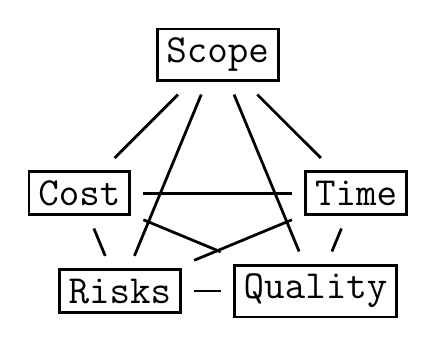
\begin{tikzpicture}[node distance=5em,
  every path/.style={draw=black, line width=.1em},
  every node/.style={font={\Large\ttfamily}, draw=black, rectangle, outer sep=.5em}]
\node[draw=none] (center) {};
\node[above of=center] (scope) {Scope};
\node[below left of=center] (risks) {Risks};
\node[below right of=center] (quality) {Quality};
\node[right of=center] (time) {Time};
\node[left of=center] (cost) {Cost};
\path (scope) -- (time);
\path (time) -- (cost);
\path (cost) -- (scope);
\path (quality) -- (time);
\path (quality) -- (cost);
\path (quality) -- (scope);
\path (risks) -- (time);
\path (risks) -- (cost);
\path (risks) -- (scope);
\path (risks) -- (quality);
\end{tikzpicture}
}

\pmbaQuestion
  {You just found out that one of your key programmers posted his resume on a job board. What do you do immediately?}
  {Nothing}
  {Update risk list}
  {Post a vacation}
  {Offer him a raise}
  {staff}

\pmbaQuestion
  {What is the cost of a risk, if \emph{probability} is 0.8, \emph{impact} is 0.7, and \emph{effect} is \pounds1,000?}
  {\pounds1,500}
  {\pounds560}
  {\pounds800}
  {\pounds700}
  {quantitative}

\pmbaQuestion
  {What is the name of a risk with a \emph{negative value} of the \emph{impact}?}
  {Opportunity}
  {Residual Risk}
  {Threat}
  {Secondary Risk}
  {register}

\pmbaQuestion
  {What is the relation of elements in the cause-risk-effect format?}
  {Many-one-many}
  {Many-many-many}
  {Many-one-one}
  {One-one-one}
  {format}

\pmbaQuestion
  {At a technical meeting, a programmer says: "I think the use of this framework will lead to problems in the future". What do you answer?}
  {``Be positive, negativity is not welcome here''} % ignore
  {``Can we prevent them?''} % mitigate
  {``OK, let's use another one''} % avoid
  {``Big problems?''} % accept
  {staff}

\pmbaQuestion
  {A new architect replaces the previous one and tells you that there is a serious security flaw in the system. What do you do?}
  {Ask him to \emph{fix} it immediately}
  {Ask him to \emph{not disclose} this information to anyone}
  {Ask him to \emph{estimate} the risk of attack}
  {Nothing}
  {identification}

\pmbaQuestion
  {The estimated duration of the project is 20 months. There is a \emph{3x9} risk that a few key engineers may leave the company soon. If this happens, the project will be delayed by another 15 months. What project duration you should report now to the customer?}
  {\(20 + 15 \times 0.3 = 24.5\)}
  {\(20 + 15 \times 0.3 + 10 = 34.5\)}
  {\(20 + 15 \times 0.3 \times 0.9 = 24.05\)}
  {\(20 + 15 = 35\)}
  {contingency, unknown-unknowns}

\pmbaQuestion
  {There is a \emph{risk} that the server will break. If this happens, a new one will cost another \$5,000. How to prepare the customer for this?}
  {Ask him to pay \$5K upfront, refund later}
  {Put \$5K into contingency reserve}
  {Put \$5K into management reserve}
  {Put \$2.5K into project budget}
  {reserves}

\plush{
  \pptBanner{Homework:}
  ``\emph{Risk Register} is a document in which the results of risk analysis and risk response planning
  are recorded. It contains the outcomes of the other risk management processes as they are
  conducted, resulting in an increase in the level and type of information contained in the
  risk register over time.'' --- PMBOK5
}

\plush{
  \pptBanner{Read this:}
  Rita Mulcahy, \textit{Risk Management, Tricks of the Trade for Project Managers}, 2003\par
  \href{https://www.yegor256.com/2019/05/14/cause-risk-effect.html}{0rsk.com: Cause + Risk + Effect} (2019)\par
  Narendra K. Shrivastava,
    \href{https://www.pmi.org/learning/library/model-risk-contingency-reserve-9310}{A model to develop and use risk contingency reserve} (2014)\par
  Elizabeth Harrin,
    \href{https://www.projectmanagement.com/blog-post/5806/management-reserves-and-contingency-reserves--what-s-the-difference-}{Management reserves and contingency reserves: what’s the difference?} (2012)\par
}

\end{document}
